\part{Solution} \label{part:solution}

\chapter{Design}

This chapter will be the occasion to detail the architecture of our solution. We will explain the technologies employed to achieve our goal, a monitoring software for Internet of Things networks. It is also in this chapter that we will justify the choices made during the development of it.

\section{Architecture}

The architecture of our solution is comprised of two parts as can be seen on Fig.\ref{fig:design}. The first part is about how the data is collected and sent. The second part consists on how the data is received and treated after reception. In the remaining of the section, strong assumptions are made that the reader is familiar with Netflow, particularly Netflow v10 or IPFIX, and also its implementation for WSN which is called TinyIPFIX. If not, explanations about those particular technologies can be found in Chap \ref{chap:monitoring_tools}. \\

\begin{figure}
	\centering
	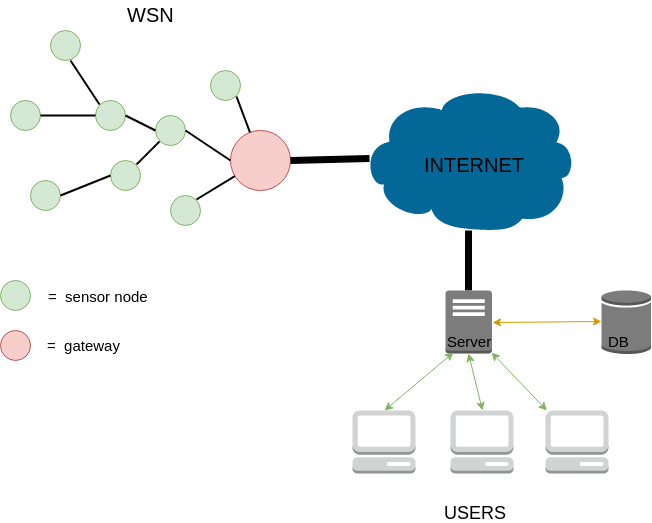
\includegraphics[width=0.8\textwidth]{res/design.png}
	\caption{Global architecture of the solution}
	\label{fig:design}
\end{figure}

The data exportation is done in a Netflow fashion. The nodes occupy the roles of exporters. Each node maintain a flow table where they register the flows that occurred during an interval of time. In our case a flow is characterized by the 4-uple: source node id, destination node id, number packets and number octets. After a certain amount of time passes, each node will construct a TinyIPFIX message based on the content of its flow table. Those messages are sent to the gateway node. The gateway node will then reformat the TinyIPFIX messages received into compliant IPFIX messages to a specific address, which will be in our case the address of a server.\\

The server which receives the IPFIX messages from the IoT network, plays two roles. One role is straightforward. It is the role of collector. Each message is collected by the server and logged in a database for further processing and analyze. The other role, is of a web server. Multiple users can know the network status by having access to web pages served by the server.
